\documentclass[conference]{IEEEtran}

\usepackage{cite}
\usepackage{amsmath,amssymb}
\usepackage{graphicx}
\usepackage{booktabs}
\usepackage{url}
\usepackage{xspace}

% Resolve figure/table assets relative to this file.
\graphicspath{{figures/}}

\title{DeFiFlowBench: Benchmarking and Improving Safe Executability in\\
Natural-Language DeFi Workflow Synthesis}

\author{%
\IEEEauthorblockN{Anonymous Authors}
\IEEEauthorblockA{Paper under review}
}

\begin{document}
\maketitle

\begin{abstract}
Natural-language interfaces for decentralized finance (DeFi) promise to
make multi-step protocol interactions accessible to non-expert users, but
they are typically evaluated only on whether the generated workflow graph
looks structurally valid. We argue that this is the wrong bar for a
high-stakes execution domain, and we study a stricter question: are
generated DeFi workflows \emph{safely executable}? We introduce
\textsc{DeFiFlowBench}, a benchmark of 120 expert-authored prompts spanning
swaps, limit orders, cross-chain transfers, and compositional tasks, with
difficulty tiers, paraphrase clusters, and adversarial cases. Each generated
workflow is scored on three nested static layers---structural validity,
executable configuration completeness, and declared safety---and on an
execution layer that runs each generated swap on a real EVM. To make scores
interpretable we bound the scale with an oracle solver (which scores $1.00$
on every layer and is on-chain safe) and null and random-node baselines
(which score $0.00$), and we validate the static safety proxy against on-chain
outcomes: on our data the proxy never certifies a workflow that then executes
unsafely. Evaluating a deterministic template, a deployed no-code DeFi
generator, and direct, constrained, few-shot, and safety-instructed
language-model baselines across two model families, we find a large and
consistent structural-to-safe gap: the best system reaches only $0.44$
structural validity and no system exceeds $0.29$ safe-executability (95\%
CI $[0.21,0.38]$). The failure modes are complementary and quantified: the
template binds no trade parameters, the deployed generator breaks required
structure, and language models parse parameters but omit safety machinery.
On-chain, direct, constrained, and few-shot configurations each execute
$10$--$13$ swaps at roughly $33\%$ self-inflicted price impact because they
wire a slippage bound but no price-impact gate. An explicit safety
instruction is the only intervention that eliminates on-chain unsafe
execution---yet still leaves most workflows structurally incomplete---showing
the gap is real but partially addressable. We release the benchmark,
baselines, execution harness, and analysis code.

\end{abstract}

\begin{IEEEkeywords}
decentralized finance, workflow synthesis, benchmarking, language models,
executable safety, smart contracts
\end{IEEEkeywords}

\section{Introduction}
\label{sec:intro}

Natural-language workflow generation is attractive for decentralized
finance (DeFi) because common user goals---token swaps, limit orders, and
cross-chain transfers---require coordinating multiple protocols and many
configuration choices. A system that turns ``swap 1 ETH to USDC with at
most 1\% slippage'' into an executable workflow could make DeFi accessible
to users who cannot write contract calls by hand.

Evaluations of such systems, however, typically stop at whether the
generated workflow, viewed as a directed graph of nodes and edges, is
structurally valid. We argue that this is the wrong bar for DeFi. A graph
that looks correct may still be unsafe or non-executable if it omits the
concrete trade parameters needed to run, ignores price-impact limits, uses
unsupported chains or tokens, or fails to gate execution against the cost
of the user's own order. In a domain where a single transaction can move
real funds irreversibly, structural validity is necessary but far from
sufficient.

This paper reframes DeFi workflow synthesis as a benchmark and measurement
problem centered on \emph{safe executability}. We evaluate generated
workflows on three nested static layers---structural validity, executable
configuration completeness, and declared safety---and, crucially, add an
execution layer that runs each generated swap on a real EVM and observes
the on-chain outcome. This lets us separate three questions that prior
evaluations conflate: does the graph have the right shape, does it carry
the parameters needed to execute, and, when executed, does it actually
behave safely?

Our central finding is that structural validity does not imply safe
executability, and the gap is large. Across a 30-prompt pilot and a range
of systems---a deterministic template baseline, a deployed no-code DeFi
generator, and direct and constrained language-model baselines on two
model families---no system produces a single statically safe-executable
workflow. On-chain, every language-model configuration executes a large
swap at roughly $33\%$ self-inflicted price impact because it sets a
slippage bound but no price-impact gate.

\paragraph{Contributions.} (1) We define a three-layer static evaluation
of DeFi workflow synthesis (structural, executable, safe) plus a
clarification axis, with safety predicates derived uniformly across
systems. (2) We add an on-chain execution layer that runs generated swaps
on a real EVM and distinguishes a slippage bound from a price-impact gate,
turning ``declared safety'' into ``observed safety''. (3) We report a
pilot over four DeFi task categories and multiple baselines, including a
deployed no-code system and two language-model families, and show that the
structural-versus-safe gap is consistent across models and visible on
chain. (4) We release the prompts, gold annotations, baselines, and
execution harness for reproducible evaluation.

\section{Problem Statement and the Safety Ladder}
\label{sec:method}

\subsection{Task}

DeFi workflow synthesis maps a natural-language intent $p$ to a workflow
specification $W = (N, E, C)$: a set $N$ of typed nodes drawn from a fixed
executable DeFi node vocabulary (e.g.\ \texttt{tokenSelector},
\texttt{oneInchQuote}, \texttt{priceImpact\-Calculator},
\texttt{oneInchSwap}, \texttt{limitOrder}, \texttt{fusionPlus},
\texttt{transactionMonitor}), a set $E \subseteq N \times N$ of type-level
data-flow edges, and an execution configuration $C$ mapping keys such as
\texttt{fromToken}, \texttt{amount}, \texttt{slippage}, and
\texttt{targetPrice} to concrete values.

Each benchmark item pairs a prompt with an expert-authored gold annotation
$(N^{\star}, E^{\star}, C^{\star}, S^{\star})$, where $S^{\star}$ is a set
of \emph{safety predicates} the workflow must satisfy to be safely
executable: a slippage bound, a price-impact gate, transaction monitoring,
a distinct bridge destination. The annotation also marks underspecified
prompts, for which the correct response is a clarification request rather
than a workflow.

\subsection{The safety ladder}
\label{sec:ladder}

We score every generated workflow on four strictly nested levels. Each
level subsumes the ones below it, so a system's position on the ladder
identifies which capability it lacks.

\paragraph{Level 1: graph-valid.} The workflow recalls every required node
type and required type-level edge, and the generator did not error. This
level is deliberately lenient: extra nodes are ignored unless they break a
required edge, matching the weak notion of ``valid'' that graph-only
evaluations reward.

\paragraph{Level 2: executable.} The workflow is graph-valid \emph{and}
every required configuration key in $C^{\star}$ holds a concrete,
non-placeholder value. A node that exists only in template mode, with no
trade amount or target price, is not executable.

\paragraph{Level 3: statically safe.} The workflow is executable
\emph{and} every required safety predicate in $S^{\star}$ is declared and
parameterized. Predicates are derived uniformly from the normalized
workflow for all systems, so no system benefits from self-reported safety.

\paragraph{Level 4: execution-safe.} Declaring a predicate does not prove
it gates execution, so the top level is measured by running the workflow.
We deploy a constant-product AMM (Uniswap-V2-style $x \cdot y = k$ with a
$0.3\%$ fee) and ERC20 tokens on an in-process EVM, seed deterministic
reserves, and submit each generated swap as a real transaction. The
harness observes the mined receipt, gas, or revert and labels the outcome
(\texttt{executed\_safe}, \texttt{reverted\_slippage},
\texttt{aborted\_price\_impact}, \texttt{unsafe\_executed},
\texttt{pending\_not\_filled}, or \texttt{not\_executable}). Execution
semantics are real (\texttt{transferFrom} calls, \texttt{require}
reverts, gas accounting); only the reserves are synthetic, a choice we
validate against mainnet in Section~\ref{sec:fidelity}.

A separate \emph{clarification axis} scores underspecified prompts, where
emitting a confidently wrong workflow is the failure mode.

\paragraph{Slippage is not price impact.} The distinction that drives our
headline result is between two protections that generators routinely
conflate. A \emph{slippage bound} sets a minimum output computed from the
already impact-adjusted quote; it protects against price movement between
quote and execution. It does nothing to stop a large order from executing
at severe \emph{self-inflicted} price impact. Only a separate
\emph{price-impact gate} does. A workflow that mines a high-impact trade
with no such gate is labeled \texttt{unsafe\_executed}.

\section{Benchmark}
\label{sec:benchmark}

\subsection{Categories and prompts}

\textsc{DeFiFlowBench} contains 120 expert-authored prompts across four
categories: token swaps (40), limit orders (30), cross-chain transfers (30),
and compositional workflows that combine primitives (20). Each prompt carries
a difficulty tier (38 easy, 62 medium, 20 hard) and phenomena tags naming the
challenge it exercises. Fifteen prompts are underspecified (e.g.\ ``help me
trade some tokens'') or contradictory (a bridge or swap whose source and
destination are identical) and are scored on a separate clarification axis;
several are adversarial in that the user waives a safety constraint the gold
annotation still requires (e.g.\ ``I don't care about slippage''). To measure
robustness to surface form independently of task difficulty, the benchmark
includes \emph{paraphrase clusters}: multiple prompts that encode the same
underlying task with different wording (spelled-out numbers, terse notation,
verbose narration, injected typos). Prompts vary from fully specified (``swap
1 ETH to USDC with at most 1\% slippage'') to schematic (``make a token swap
app for UNI to ETH'').

\paragraph{Held-out test split.} To measure generalization rather than
in-distribution fit, we author a separate $87$-prompt held-out split
\emph{after} freezing the Koan-Safe method (Section~\ref{sec:koansafe}) and
evaluate every system on it exactly once. It is harder in two independent
ways. First, its canonical-structure prompts use fresh surface forms and a few
\emph{out-of-vocabulary} token symbols (MKR, SUSHI, GRT) absent from
Koan-Safe's token dictionary, stressing intent extraction and clarification.
Second, a large block requires \emph{new workflow structures} not covered by
any system's category presets---a gasless/Fusion swap, a quote-first limit
order, a dashboard-augmented bridge, and a genuine cross-chain swap---each with
its own gold annotation. Because these structures lie outside Koan-Safe's fixed
presets, the split directly tests whether the method generalizes beyond the
structures it was built around. A $30$-prompt development \emph{pilot} split is
also retained for reference.

\subsection{Gold annotations}

Each prompt is paired with a gold annotation recording (i) the required
node types, (ii) the required type-level edges, (iii) the required
execution-configuration keys, (iv) the safety predicates that must hold,
and (v) a set of \emph{allowed extra nodes} that a richer-but-correct
workflow may include without penalty. The annotation scheme, including
what qualifies as a required node, edge, configuration key, and safety
predicate, is documented in the artifact's annotation guide so that the
final split can be extended consistently. The node vocabulary is taken
from an existing executable DeFi node catalog, ensuring every required
node corresponds to a real executor rather than an abstract label.

\subsection{Baselines}

We evaluate three reference baselines that calibrate the scale and five
system families, all scored by the identical evaluator:

\begin{itemize}
  \item \textbf{Oracle (ceiling).} Reconstructs a correct workflow from the
        gold annotation---required nodes and edges, concrete values for every
        required configuration key, and the parameters needed for
        \texttt{derive\_safety} to declare each required predicate. It should,
        and does, score $1.00$ on every layer, proving the tasks are solvable
        and the scorer rewards a correct solution.
  \item \textbf{Null and Random (floor).} The null baseline emits an empty
        workflow; the random baseline emits a random-size sample of real nodes
        in a random chain with no configuration. Both establish the floor and
        guard against a gameable metric.
  \item \textbf{Template-only.} Emits the canonical workflow for the prompt's
        category with static safety defaults, but performs no language
        understanding and cannot populate trade-specific configuration.
  \item \textbf{Koan.} The regex-fallback intent parser and workflow generator
        of an existing no-code DeFi platform, run offline and
        deterministically---a real deployed system, not a strawman.
  \item \textbf{Direct / Constrained / Few-shot / Safety-instructed LLM.} A
        language model prompted to emit a workflow graph and configuration as
        JSON. The variants differ only in the prompt: no constraints; injected
        per-category structural and safety constraints; a single worked
        in-context example; and an explicit instruction to make the workflow
        safe to execute. Comparing the variants on a fixed model isolates the
        effect of each prompt-design intervention.
  \item \textbf{Koan-Safe (proposed).} Our safety-enforcement system
        (Section~\ref{sec:koansafe}), evaluated with all three generators
        (rule-based, LLM, hybrid) and with the enforcement layer toggled off as
        an ablation. It is scored by the identical evaluator and, like every
        other system, reads only the raw prompt text.
\end{itemize}

The LLM baselines are evaluated on two model families to test whether findings
are model-specific. Model outputs are normalized (node and edge vocabularies
filtered; index-based and name-based edge encodings both accepted) before
scoring, and each raw model response is retained so that metrics can be
re-derived deterministically without additional queries. Every reported rate
is accompanied by a 95\% Wilson confidence interval, and mean-valued metrics
by a bootstrap interval.

\section{Koan-Safe: Safety as Enforcement}
\label{sec:koansafe}

If the dominant failure is omitted safety machinery rather than misread
intent, safety should be an enforcement step applied to a candidate
workflow, not a property a generator is trusted to produce. Koan-Safe
factors synthesis into three replaceable stages: an intent parser, a
candidate generator, and a generator-agnostic safety-enforcement layer.
The factoring lets the enforcement layer be toggled and measured in
isolation.

A note on naming: \emph{Koan} is the existing deployed platform we
evaluate as a baseline; \emph{Koan-Safe} is the method proposed here;
\textsc{DeFiFlowBench} is the benchmark.

\paragraph{Intent parser.} A deterministic, prompt-only parser maps the
request text to a typed intent: task category, the trade-intent fields it
can extract (tokens, amount, slippage, target price, chains), and a
decision to build or ask for clarification. It reads only the prompt
string, never the gold annotation or category label, so it has exactly
the information available to the LLM baselines. Clarification fires only
when acting would require guessing trade intent: no recognizable token,
identical source and destination, or a bridge with no destination.

\paragraph{Candidate generator.} Three interchangeable generators feed
the same enforcement layer. \emph{Rules} emits a category-appropriate
node graph and fills configuration from the parsed intent. \emph{LLM}
uses the same neural backend as the direct baseline. \emph{Hybrid} takes
the LLM's structure but backfills trade-intent configuration that the
parser read from the prompt and the model dropped.

\paragraph{Safety-enforcement layer.} Given any candidate workflow and
the parsed intent, the layer repairs structure by adding the category's
required safety nodes and reconnecting the required spine, then injects
conservative safety policy the request did not pin down: a default
slippage bound, a price-impact gate with a concrete threshold, a bridge
confirmation count, a default order expiry, and a self-recipient for
bridges. The layer never fabricates trade intent. It adds no token,
amount, target price, or chain absent from the request, so a prompt that
omits an amount yields a structurally valid but non-executable workflow
rather than an invented trade. A safety waiver in the prompt (``I don't
care about slippage'') is deliberately overridden: a safe system must
refuse to ship an unsafe trade even when asked.

\paragraph{Integrity of the comparison.} Koan-Safe encodes engineered
domain knowledge (a token dictionary, per-category node presets,
conservative safety defaults) but has no access to gold annotations.
Because its structural presets are fixed, the held-out split deliberately
requires workflow structures outside those presets, so generalization is
tested rather than assumed.

\section{Experimental Setup}
\label{sec:setup}

Our experiments answer three research questions:
\begin{itemize}
  \item \textbf{RQ1}: Do graph-valid DeFi workflows fail to be safely
        executable, and how does the failure manifest on-chain?
  \item \textbf{RQ2}: Does Koan-Safe improve safe executability on a
        held-out split with novel workflow structures?
  \item \textbf{RQ3}: Is the enforcement layer, rather than the parser or
        generator, causally responsible?
\end{itemize}

\paragraph{Splits.} The development split (120 prompts; $n=105$ workflow
prompts after removing the clarification subset) is where Koan-Safe was
built and tuned. The held-out test split (87 prompts; $n=75$) was
authored after Koan-Safe was frozen and evaluated exactly once. Unless
noted, all results report the held-out split.

\paragraph{Models and reproducibility.} LLM systems run at temperature
$0$ on Gemini~3.1~Flash~Lite and GPT-5.4~mini through a common OpenRouter
endpoint. Temperature-$0$ API calls still vary slightly across runs, so
exact decimals may shift on re-run; all tables are generated from saved
outputs, and every raw model response is stored. Every rate carries a
95\% Wilson confidence interval; mean-valued metrics carry a bootstrap
interval.

\paragraph{Calibration.} The oracle scores $1.00$ on every static level
and is safe on every executed swap on both splits, so the tasks,
including the held-out structural variants, are solvable and the scorer
rewards a correct solution. The null and random-node floors score $0.00$
on every level, so the metric cannot be gamed by degenerate or padded
graphs (Table~\ref{tab:main-results}).

\section{Results}
\label{sec:results}

\begin{table}[t]
\centering
\caption{Static structural/executable/safe metrics vs.\ on-chain execution on the pilot split ($n{=}26$ workflow prompts). Fork-Unsafe counts workflows that executed on a local py-EVM at $>$5\% own-trade price impact with no price-impact gate. LLM baselines run at temperature~0.}
\label{tab:main-results}
\begin{tabular}{lccccc}
\toprule
System & Graph & Exec. & Safe & Fork & Fork \\
       & valid & (cfg) & (cfg) & unsafe & safe-rate \\
\midrule
Template-only & 1.00 & 0.00 & 0.00 & 0 & n/a \\
Koan (regex$+$gen) & 0.15 & 0.00 & 0.00 & 0 & n/a \\
Direct LLM (Gemini 3.1 FL) & 0.08 & 0.04 & 0.00 & 1 & 0.67 \\
Direct LLM (GPT-5.4 mini) & 0.04 & 0.00 & 0.00 & 1 & 0.50 \\
Constrained LLM (Gemini 3.1 FL) & 0.27 & 0.04 & 0.00 & 1 & 0.67 \\
Constrained LLM (GPT-5.4 mini) & 0.04 & 0.00 & 0.00 & 1 & 0.50 \\
\bottomrule
\end{tabular}
\end{table}


\begin{figure*}[t]
\centering
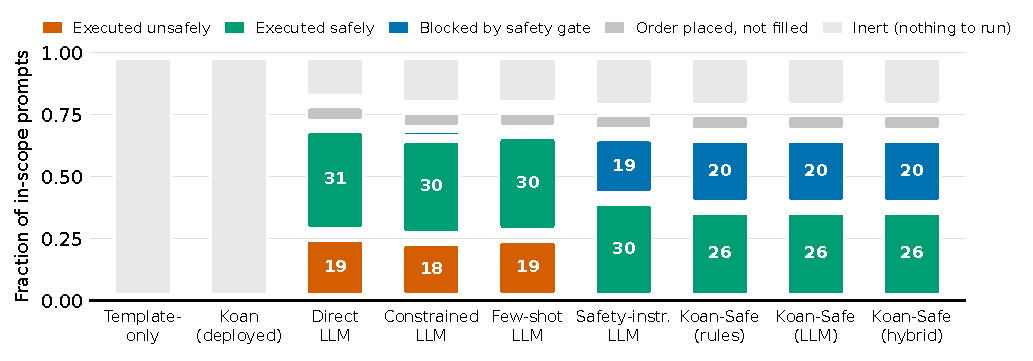
\includegraphics[width=\textwidth]{onchain_fates.pdf}
\caption{\textbf{Two ways to be ``safe'': gated, or inert.} On-chain fate
of every in-scope prompt on the local EVM (cross-chain prompts, which a
single local chain cannot bridge, are excluded). The template and
deployed-Koan baselines are harmless only because they are inert: nothing
they emit can execute. The direct, constrained, and few-shot LLMs execute
readily and mine $18$--$19$ swaps unsafely (orange). Koan-Safe executes
just as often, but its injected price-impact gate blocks the $20$
dangerous trades (blue) instead of mining them. LLM systems shown on
Gemini~3.1~FL; GPT-5.4~mini rows appear in Table~\ref{tab:main-results}.}
\label{fig:fates}
\end{figure*}

\begin{figure}[t]
\centering
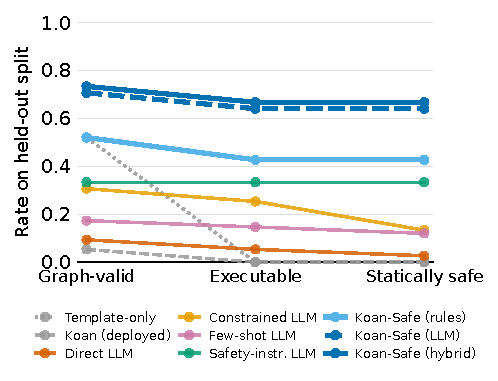
\includegraphics[width=\columnwidth]{safety_ladder.pdf}
\caption{Survival across the static safety-ladder levels on the held-out
test split ($n{=}75$). Baselines (grey/warm) collapse between levels;
Koan-Safe (blue) starts high and loses nothing at the safety step.}
\label{fig:ladder}
\end{figure}

\subsection{RQ1: Structural validity does not imply safe executability}
\label{sec:rq1}

On the held-out split \textbf{no baseline exceeds $0.33$
safe-executability} (safety-instructed Gemini, 95\% CI $[0.24,0.45]$),
and most sit near the floor (Table~\ref{tab:main-results},
Figure~\ref{fig:ladder}). Each system falls off the ladder at a
diagnostic rung. The template baseline is graph-valid on canonical
prompts ($0.52$) but has zero configuration completeness: well-formed
graphs with no executable trade. The deployed Koan generator is
graph-valid on only $0.05$ of prompts, over-generating into a fixed suite
that breaks required structure. The LLM baselines invert the trade-off:
they extract concrete configuration but omit safety machinery.

On-chain, these failure modes produce two very different kinds of
``zero unsafe executions'' (Figure~\ref{fig:fates}). The
template and Koan baselines are harmless only because they are inert;
nothing they emit can execute. The LLM baselines are the opposite. Under
direct, constrained, and few-shot prompting, both model families emit
swaps with a concrete amount but no wired price-impact gate, and these
\textbf{mine at roughly $33\%$ self-inflicted price impact}: $15$ to
$19$ \texttt{unsafe\_executed} outcomes per configuration. The slippage
bound the models do set never fires, because its minimum output is
computed from the already impact-adjusted quote. A useful system must be
neither inert nor ungated, and no baseline manages both.

Prompting alone does not close the gap. Structural constraints and a
few-shot example raise graph validity but leave $17$--$19$ unsafe
executions intact. An explicit safety instruction eliminates unsafe
execution on both models by inducing a parameterized gate, yet leaves
most workflows structurally incomplete ($0.33$ Gemini, $0.07$ GPT).
Safety parameterization is promptable; robust structure is not.

\subsection{RQ2: Koan-Safe doubles held-out safe executability}
\label{sec:rq2}

All three Koan-Safe generators lead the held-out split. The hybrid
generator on Gemini reaches $0.67$ safe-executability (95\% CI
$[0.55,0.76]$), \textbf{double the best baseline}, with the LLM generator
at $0.64$ and rules at $0.43$. Its zero unsafe executions are of the
useful kind: Koan-Safe executes about as often as the plain LLM baselines
($26$ safe executions vs.\ their $30$--$31$), but the $20$ trades that
would have mined at high impact are blocked by the injected price-impact
gate (Figure~\ref{fig:fates}). Every Koan-Safe configuration, on both
model families, records zero on-chain unsafe executions.

The generator split exposes a limitation and its remedy. The frozen
rule-based presets do not cover the held-out structural variants, so
rules falls from $1.00$ structural validity on development to $0.52$.
The LLM generator, unconstrained by presets, generalizes to the variants
(graph-valid $0.71$); the hybrid does best ($0.73$). On development,
where presets match, all three generators reach $1.00$ structural
validity and $0.55$--$0.58$ safe-executability. In every case the
enforcement layer converts whatever structure it is given into on-chain
safety.

On the clarification axis, Koan-Safe correctly handles $9$ of $12$
underspecified or contradictory prompts; the three misses are terse
requests (``I want a limit order'') that its frozen decision rule builds
instead of questioning. Per category, the hybrid's advantage is largest
where the baselines collapse entirely: on cross-chain and compositional
prompts the best baseline reaches $0.07$ safe-executability while the
hybrid reaches $0.72$ and $0.42$; on limit orders it is perfect
($1.00$ vs.\ $0.53$). Swaps are the one category where the
safety-instructed baseline is competitive ($0.61$ vs.\ $0.54$).

\subsection{RQ3: The enforcement layer is the cause}
\label{sec:rq3}

Toggling only the enforcement layer, with parser and generator fixed,
collapses safe-executability for every generator: rules $0.43 \to 0.12$,
LLM $0.64 \to 0.00$, hybrid $0.67 \to 0.01$
(Table~\ref{tab:enforcement-ablation}). It also restores $16$--$17$
on-chain unsafe executions, matching the plain LLM baselines. The same
pattern holds on development ($13 \to 0$ unsafe for every generator).
Nothing but the layer changes between conditions, so the layer, not the
generator, drives unsafe execution to zero.

\begin{table}[t]
\centering
\caption{Enforcement-layer ablation on the heldout split: each Koan-Safe generator with the safety-enforcement layer on vs.\ off (same parser and generator). The layer is what drives on-chain unsafe executions to zero.}
\label{tab:enforcement-ablation}
\begin{tabular}{lcccc}
\toprule
System & \multicolumn{2}{c}{Safe (cfg)} & \multicolumn{2}{c}{Fork unsafe} \\
 & off & on & off & on \\
\midrule
Koan-Safe (rules) & 0.12 & 0.43 & 17 & 0 \\
Koan-Safe (LLM) (Gemini 3.1 FL) & 0.00 & 0.64 & 17 & 0 \\
Koan-Safe (hybrid) (Gemini 3.1 FL) & 0.01 & 0.67 & 16 & 0 \\
\bottomrule
\end{tabular}
\end{table}


\subsection{Robustness: metamorphic safety without labels}
\label{sec:metamorphic}

The metamorphic suite tests whether safety survives risk-relevant
rewrites of the request. The direct LLMs violate $14$--$16$ of
${\sim}32$ applicable relations (Table~\ref{tab:metamorphic}),
concentrated where RQ1 predicts: they fail every amount-monotonicity
pair, silently executing the $100\times$ larger trade at severe impact,
and comply with $6$--$7$ of $8$ waivers by dropping the protections the
base request had. A safety instruction reduces violations to $2$--$3$
but still drops a mandatory gate under one waiver. \textbf{Every
Koan-Safe configuration satisfies all amount, threshold, waiver, and
drop-field relations on both models}; the single residual is one
paraphrase pair where the hybrid's LLM structure step emits a different
class for a cross-chain rewording. Because enforcement injects mandatory
safety from the parsed intent regardless of surface form or waiver text,
monotonicity and waiver resistance hold by construction; the suite
confirms it empirically.

\begin{table*}[t]
\centering
\caption{Metamorphic safety violations (count of violated pairs, lower is better) by relation on the metamorphic suite. Amount: $100\times$ larger trade must not weaken safety; Thr: tightening tolerance must keep the gate; Waiv: an explicit safety waiver must not remove mandatory gates; Para: paraphrase must preserve class and policy; Drop: a removed field must not be fabricated. Denominators vary because pairs whose base prompt a system fails to build are not applicable.}
\label{tab:metamorphic}
\begin{tabular}{lcccccc}
\toprule
System & Amt & Thr & Waiv & Para & Drop & All \\
\midrule
Direct LLM (GPT-5.4 mini) & 7 & 0 & 7 & 2 & 0 & 16/33 \\
Direct LLM (Gemini 3.1 FL) & 8 & 0 & 6 & 0 & 0 & 14/32 \\
Safety-instruct LLM (GPT-5.4 mini) & 0 & 1 & 0 & 1 & 0 & 2/28 \\
Safety-instruct LLM (Gemini 3.1 FL) & 0 & 0 & 1 & 2 & 0 & 3/30 \\
Koan-Safe (rules) & 0 & 0 & 0 & 0 & 0 & 0/34 \\
Koan-Safe (LLM) (GPT-5.4 mini) & 0 & 0 & 0 & 0 & 0 & 0/34 \\
Koan-Safe (LLM) (Gemini 3.1 FL) & 0 & 0 & 0 & 0 & 0 & 0/34 \\
Koan-Safe (hybrid) (GPT-5.4 mini) & 0 & 0 & 0 & 0 & 0 & 0/34 \\
Koan-Safe (hybrid) (Gemini 3.1 FL) & 0 & 0 & 0 & 1 & 0 & 1/34 \\
\bottomrule
\end{tabular}
\end{table*}


\subsection{Cost and latency}
\label{sec:cost}

Enforcement is effectively free. The rule-based generator makes zero LLM
calls; the LLM and hybrid generators make one call per built workflow,
slightly fewer than the baselines because the clarification gate fires
before generation ($0.99$ vs.\ $1.00$ calls/workflow). End-to-end latency
is dominated by provider round-trip (${\sim}1.7$--$2.0$\,s) and
indistinguishable between Koan-Safe and the baselines; the enforcement
layer's own overhead is $0.07$\,ms per workflow. At \$0.30 per million
output tokens the spend is under \$0.005 per 100 workflows for every
system.

\section{Analysis}
\label{sec:analysis}

\subsection{Construct validity: does the static proxy measure real safety?}

The static safe-executable layer is a cheap proxy for an expensive property:
whether a workflow is actually safe to run. We test the proxy against the
on-chain outcome on every prompt the fork harness executed or gated to a
definite safe/unsafe label ($n=891$ system$\times$prompt pairs on the held-out
split). The proxy is \emph{sound} on this data: of the $282$ workflows it
declares safe-executable, all $282$ are safe on-chain---\emph{precision
$1.00$, zero false certifications}. Because Koan-Safe actually parameterizes a
price-impact gate, these are genuine true positives, not an artifact of no
system ever declaring safety (as was the case for the baselines alone). The
proxy is also deliberately conservative: in $453$ pairs it withholds ``safe''
from a workflow whose single executed swap happened to be within impact bounds,
because it requires a declared gate rather than a fortunate trade size. The
$156$ proxy-unsafe/on-chain-unsafe pairs are the concrete unsafe executions it
correctly refuses to certify. This is the intended direction of error for a
safety metric: it never certifies danger as safe.

\subsection{Failure taxonomy}

Aggregating the per-prompt scores into named failure categories (released in
full with the artifact) separates the systems' error profiles on the held-out
split. The deployed Koan generator's failures are structural: $71$ missing
required edges and $54$ missing required nodes, driven by fixed-suite
over-generation. The LLM baselines' failures are predominantly
\emph{safety-predicate} omissions: for direct Gemini the most frequent missing
predicate is \texttt{price\_impact\_gate} ($43$ prompts), followed by
\texttt{transaction\_monitoring} ($32$) and \texttt{bridge\_confirmation}
($15$). Koan-Safe's enforcement layer targets exactly these: the hybrid
generator's remaining errors are almost entirely structural
(\texttt{missing\_required\_edge}~$20$, driven by the held-out structural
variants) with only $8$ residual safety-predicate omissions in total, since
the layer injects the safety policy the generator would otherwise omit.

\subsection{Robustness to surface form and difficulty}

The development split holds task semantics fixed across paraphrase clusters and
tags each prompt with a difficulty tier, letting us separate competence from
surface sensitivity. On development, within-cluster graph-valid agreement is
high for Koan-Safe (rule-based $1.00$) because enforcement makes structure
deterministic, and lower for constrained Gemini ($0.81$), indicating that some
of the LLM baseline's structural score is surface-sensitive. Across difficulty
tiers on the held-out split, the hybrid generator degrades gracefully (easy
$1.00$, medium $0.77$, hard $0.25$) and dominates the constrained-LLM baseline
at every tier (easy $0.56$, medium $0.26$, hard $0.17$); the hard tier is
dominated by the novel structural variants, where the frozen rule-based
generator falls furthest (hard $0.25$) and the neural generators recover most
of the loss.

\section{Related Work}
\label{sec:related}

\paragraph{Workflow and agentic generation benchmarks.} Recent work
evaluates whether language models can generate multi-step workflows.
WorFBench~\cite{worfbench2025} benchmarks agentic workflow generation and
scores generated workflows largely at the level of graph structure and
node/edge correctness. Our work is complementary but distinct: we argue
that for a high-stakes execution domain such as DeFi, graph-level
correctness is necessary but insufficient, and we add executable and
on-chain safety layers on top of structural scoring.

\paragraph{Tool-use and API evaluation.} A related line evaluates LLMs as
tool users. ToolLLM~\cite{toolllm2024} and
API-Bank~\cite{apibank2023} measure whether models can select and invoke
external APIs to satisfy instructions. These benchmarks emphasize correct
API selection and invocation; they do not model domain-specific safety
predicates such as price-impact gating, nor do they execute the resulting
plans against a stateful financial system. We adopt the tool-use framing
but specialize the evaluation to safety-constrained on-chain execution.

\paragraph{Decentralized finance and automated market makers.} Our
execution layer builds on the constant-product automated market maker
design introduced by Uniswap~\cite{uniswapv2}, whose $x\cdot y = k$
invariant makes price impact an explicit, computable function of trade
size. This is precisely the property that lets us distinguish a slippage
bound from a price-impact gate and observe unsafe execution directly.

\paragraph{No-code DeFi workflow systems.} We evaluate an existing no-code
DeFi platform (Koan) as a first-class baseline rather than a strawman,
using its real intent parser and workflow generator. To our knowledge,
prior no-code DeFi tooling has not been evaluated against an executable
safety benchmark, which is the gap this paper addresses.

\section{Limitations}
\label{sec:limitations}

\paragraph{Local EVM, not live-fund execution.} All execution runs
against the local in-process chain; the mainnet interaction in
Section~\ref{sec:fidelity} is read-only state fetching. We never submit
transactions to a live network or move real funds. Extending the harness
to a full mainnet-fork node, with real routing and multi-hop paths, is a
natural next step.

\paragraph{Scale, single annotator, and scoring strictness.} The
development split has 120 prompts and the held-out split 87, with a
single temperature-$0$ run per model on two model families. The gold
annotations were authored primarily by one team; we provide a
second-annotator protocol, a stratified subset, and tooling to compute
inter-annotator agreement, but the agreement number awaits an independent
pass and is not yet reported. Edge matching is strict and type-level,
which penalizes reasonable-but-reordered graphs and makes structural
rates a lower bound. This does not affect the unsafe-execution findings,
which are driven by missing safety parameterization rather than edge
ordering.

\paragraph{Scope of the Koan-Safe method.} The enforcement layer improves
safety, not intent extraction: it never fabricates a missing amount,
price, or chain, so its achievable executable rate is bounded by what the
parser and generator read from the prompt. The rule-based generator's
fixed presets do not cover structures outside the four categories, which
the held-out variants expose; the LLM and hybrid generators mitigate but
do not fully remove this. The held-out split was authored by the same
team as the method, so it tests structural and surface generalization but
not adversarial distribution shift from an independent party.

\paragraph{Category scope of the execution layer.} On-chain execution
covers swaps and the swap leg of compositional workflows. Limit orders
are checked for immediate fillability against the pool mid-price, and
cross-chain workflows are not executed because a single local chain
cannot bridge. Every unexecuted case is recorded explicitly rather than
silently passed.

\section{Ethics and Responsible Disclosure}
\label{sec:ethics}

This work is an offline evaluation: no transaction in this paper touches
a live network or real funds. The benchmark is intended to help identify
unsafe generated workflows before execution, not to encourage executing
generated DeFi workflows with real assets. The evaluated no-code system
and the language models are used as-is through their public interfaces;
we report their failures to motivate safer synthesis, not to single out
any implementation. Model outputs and derived metrics are released so
the results can be independently reproduced and audited.


\section*{Acknowledgements}
AI language model assistance was used for grammatical and stylistic edits
to the text. All experiments, code, datasets, gold annotations, and
quantitative results were designed, implemented, and verified by the
authors.

\bibliographystyle{IEEEtran}
\bibliography{references}

\end{document}
